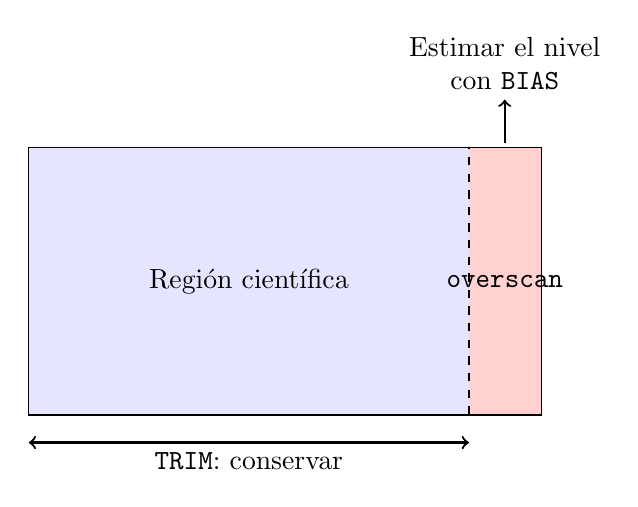
\begin{tikzpicture}[x=0.65cm,y=0.65cm]
  \draw[thick] (0,0) rectangle (10,5.2);
  \fill[blue!10] (0,0) rectangle (8.6,5.2);
  \fill[red!18] (8.6,0) rectangle (10,5.2);
  \draw[thick,dashed] (8.6,0) -- (8.6,5.2);
  \node[align=center] at (4.3,2.6) {Región científica};
  \node[align=center] at (9.3,2.6) {\texttt{overscan}};
  \draw[<->,thick] (0,-0.55) -- (8.6,-0.55)
    node[midway,below] {\texttt{TRIM}: conservar};
  \draw[->,thick] (9.3,5.3) -- (9.3,6.15)
    node[above,align=center] {Estimar el nivel\\con \texttt{BIAS}};
\end{tikzpicture}